\documentclass[addpoints,12pt,twoside]{exam} %answers 
\usepackage[paper=a4paper,left=15mm,right=15mm,top=25mm,bottom=25mm]{geometry}
\usepackage{graphicx}
%\usepackage[dvips]{graphicx}
\usepackage{floatflt,epsfig} 
\usepackage{ngerman}
\usepackage{german}
\usepackage[utf8]{inputenc}
\usepackage{amssymb, amsmath}
\usepackage[gate,ic,optics]{circ}
\usepackage{hyperref}

\usepackage{tikz,pgfplots}

\usepackage{graphicx}
%\usepackage{geometry}
\usepackage{calc}


\usepackage{qrcode} 
\usepackage{wrapfig}
\usepackage{gensymb}
\usepackage{siunitx}

\usepackage{color}
\definecolor{GridColor}{gray}{0.8}
\definecolor{SolutionBoxColor}{gray}{0.8}
\definecolor{SolutionColor}{rgb}{0.8,0.9,1}

\colorgrids
\colorsolutionboxes

%%%%%%%%%%%%%%%%%%%%%%%% MACROS %%%%%%%%%%%%%%%%%%%%%%%%%
\newcommand{\tdate}{18. April 2021}
\newcommand{\myqr}{\qrcode[hyperlink, height = 1cm]{www.github.com/shahrrks}}
\newcommand\gauss[2]{1/(#2*sqrt(2*pi))*exp(-((x-#1)^2)/(2*#2^2))} % Gauss function, parameters mu and sigma
\newcommand{\drawgraph}{ 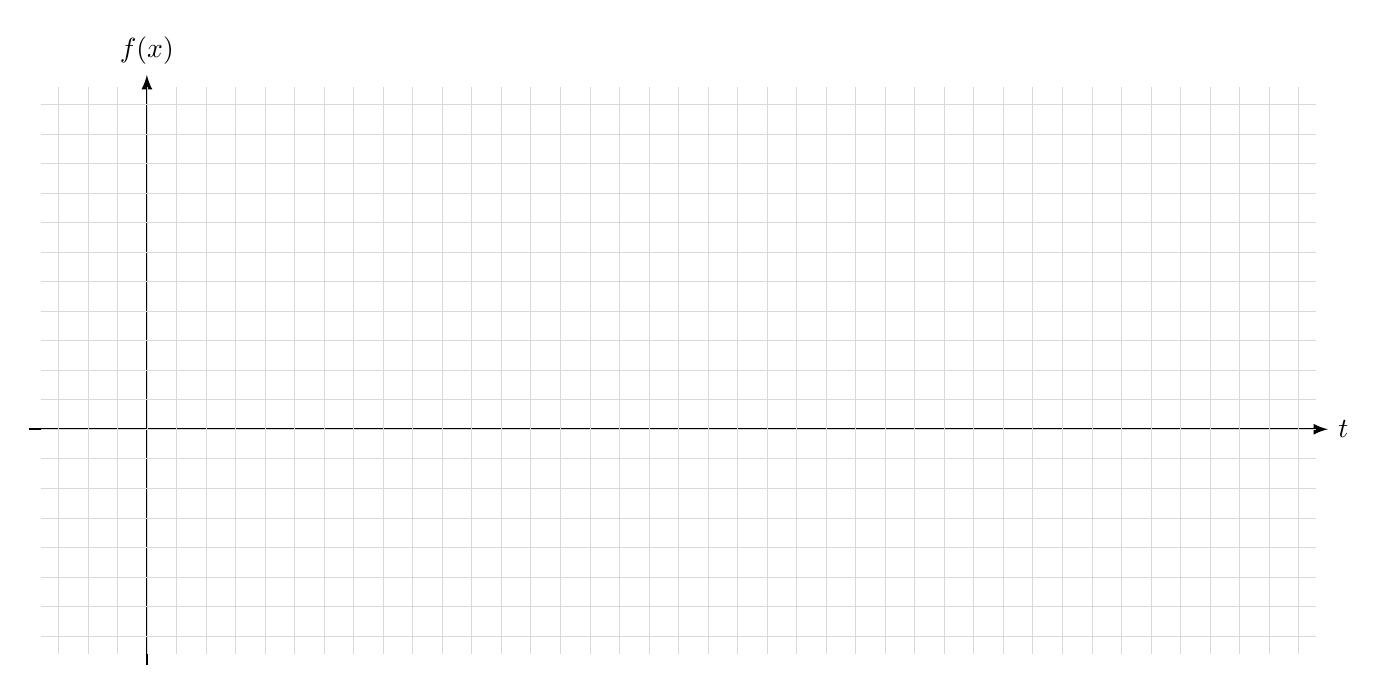
\begin{tikzpicture}[scale = 1.5]
	\draw[style = thick, -latex] (-4,0) -- (7,0) node[right] {\( t  \)};
	\draw[style = thick, -latex](-3,-2) -- (-3,3) node[above]{\( f(x)  \)};
	\draw[step=.25cm,gray!30,very thin] (-3.9,-1.9) grid (6.9,2.9);

\end{tikzpicture}}
%%

\sisetup{
	locale = DE ,
	per-mode = symbol
}

\pagestyle{headandfoot}

\headrule
\footrule
\firstpageheader{ETIT-4}{\bfseries\Large {Übungsblatt 1}}{\tdate}
\runningheader{ETIT-4}
{Übungsblatt - 1}
{\tdate}
\firstpagefooter{ETIT-4}{Seite \thepage\ von \numpages}{\myqr}
\runningfooter{ETIT-4}{Seite \thepage\ von \numpages}{Shah Rrks}

\boxedpoints
%\pointpoints{Punkt}{Punkte}
\pointsinmargin
\marginpointname{\%}

\begin{document}
	%\setcounter{section}{1} %current page -1
	\author{Shah Rrks}
	\section*{Sys 1}
	\begin{questions}
		\question[5]
		Zeichnen sie die folgende Signale als Funktion: 
		\[
		x(t) = 2 + \cos\bigg(\frac{\pi t}{2s} + \pi\bigg)
		\]
		
		\drawgraph
		
		\question[5]
		\[
		x(t) = 5e^{-t/0.5T}.\varepsilon (t)
		\]
		
		
		\drawgraph 
		
		\newpage
		\question[5]
		\[ x(t) = \frac{2}{T}.rect\bigg(\frac{T-T/2}{T/2}\bigg)
		\]
		\drawgraph
		\question[10]
		Schreiben sie einen Matlab code, der diese Funktion als ein Plot darstellt. 
		\makeemptybox{4in}
		\qrcode[height = 1cm]{https://www.youtube.com/channel/UCiHSFpMlrhxuYAIA52aLu3w}
		
		\newpage
	
	\section*{Info2}
	Boolsche Algebra Übungen (quelle:\url{ocw.mit.edu})
	\begin{figure}[h]
		\centering
		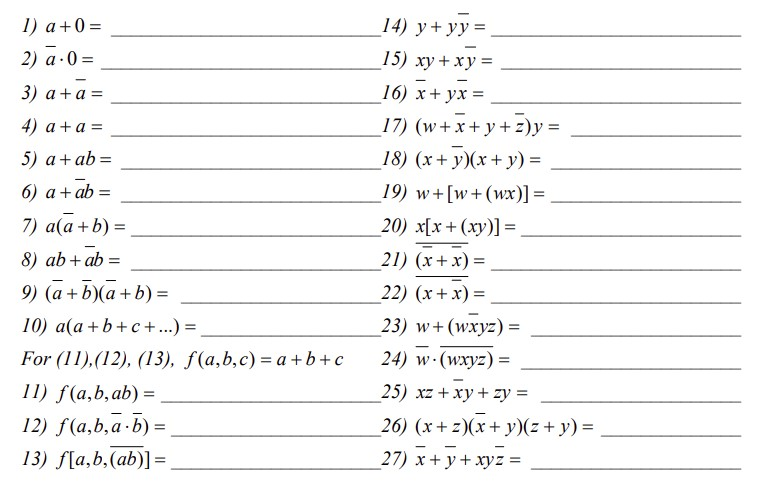
\includegraphics[width=1\linewidth]{bool_algebra}
	%	\caption{}
	\label{fig:boolalgebra}
	\end{figure}
\qrcode[hyperlink,height = 1cm]{https://github.com/shahrrks/Tutorium-ETIT-4-/blob/main/Formeln_zettel/} \hspace{5cm}
\qrcode[height = 1cm]{http://web.mit.edu/6.111/www/s2007/PSETS/pset1s.pdf}
\end{questions}
\end{document}
